% 
% Licensed to the Apache Software Foundation (ASF) under one
% or more contributor license agreements.  See the NOTICE file
% distributed with this work for additional information
% regarding copyright ownership.  The ASF licenses this file
% to you under the Apache License, Version 2.0 (the
% "License"); you may not use this file except in compliance
% with the License.  You may obtain a copy of the License at
% 
%   http://www.apache.org/licenses/LICENSE-2.0
% 
% Unless required by applicable law or agreed to in writing,
% software distributed under the License is distributed on an
% "AS IS" BASIS, WITHOUT WARRANTIES OR CONDITIONS OF ANY
% KIND, either express or implied.  See the License for the
% specific language governing permissions and limitations
% under the License.
% 

\section{DUCC Database Integration}

    DUCC is integrated with the Apache Cassandra database (\url{https://cassandra.apache.org/}.  As of
    DUCC release 2.1.0 the database is used for the following functions:
    \begin{itemize}
      \item History.  Previously a history file for all work in the system was written to the
        DUCC {\em history} directory.  These files are now written to the database.  As of this
        writing, we write the serialized DUCC objects as blobs for future reference with
        several tables summarizing the contents of the blob for use by command-line utilities
        and the webserver.
     \item Service registry.  Previously, the service registry was maintained as a collection of
       Java {\em properties} files in the DUCC {\em state} directory.  As of 2.1.0, the registry
       is maintained in a set of database tables.
    \item Service registry history.  Previously, when a service was unregistered, it's registry
      files were moved to the DUCC {\em history} directory.  As of 2.1.0, a property in
      the database tables for the registry is updated to indicate the entry is archived.
    \item Orchestrator checkpoint.  Previously, the DUCC Orchestrator would write a file
      containing the state of all active work in the system, used for restart of the system.  
      As of 2.1.0, this checkpoint file is written as a BLOB to the database.
    \item Resource Manager dynamic state.  Previously, this was not persisted.  As of 2.1.0,
      the current state of all hosts in the system, and all work scheduled on these hosts
      is maintained in the database.  This state is deleted when the RM starts, and is rebuilt
      or updated as nodes check in to the RM and as work enters and leaves.
    \end{itemize}

\section{Code Organization}

    \paragraph{Dependencies} All code that interfaces with the database resides in a single project,
    in a single directory in the DUCC source, {\em uima-ducc-database}.  All access to this function
    by the DUCC daemons is through interfaces.  There are no compile-time dependencies on this
    project by other DUCC projects; conversely, this project has compile-time dependencies only on
    the low-level common code: {\em uima-ducc-common, uima-ducc-transport, and uima-ducc-user}.
    
    Figure ~\ref{fig:db-structure} provides a visual overview of the Database component structure.
    \begin{figure}[H]
      \centering
      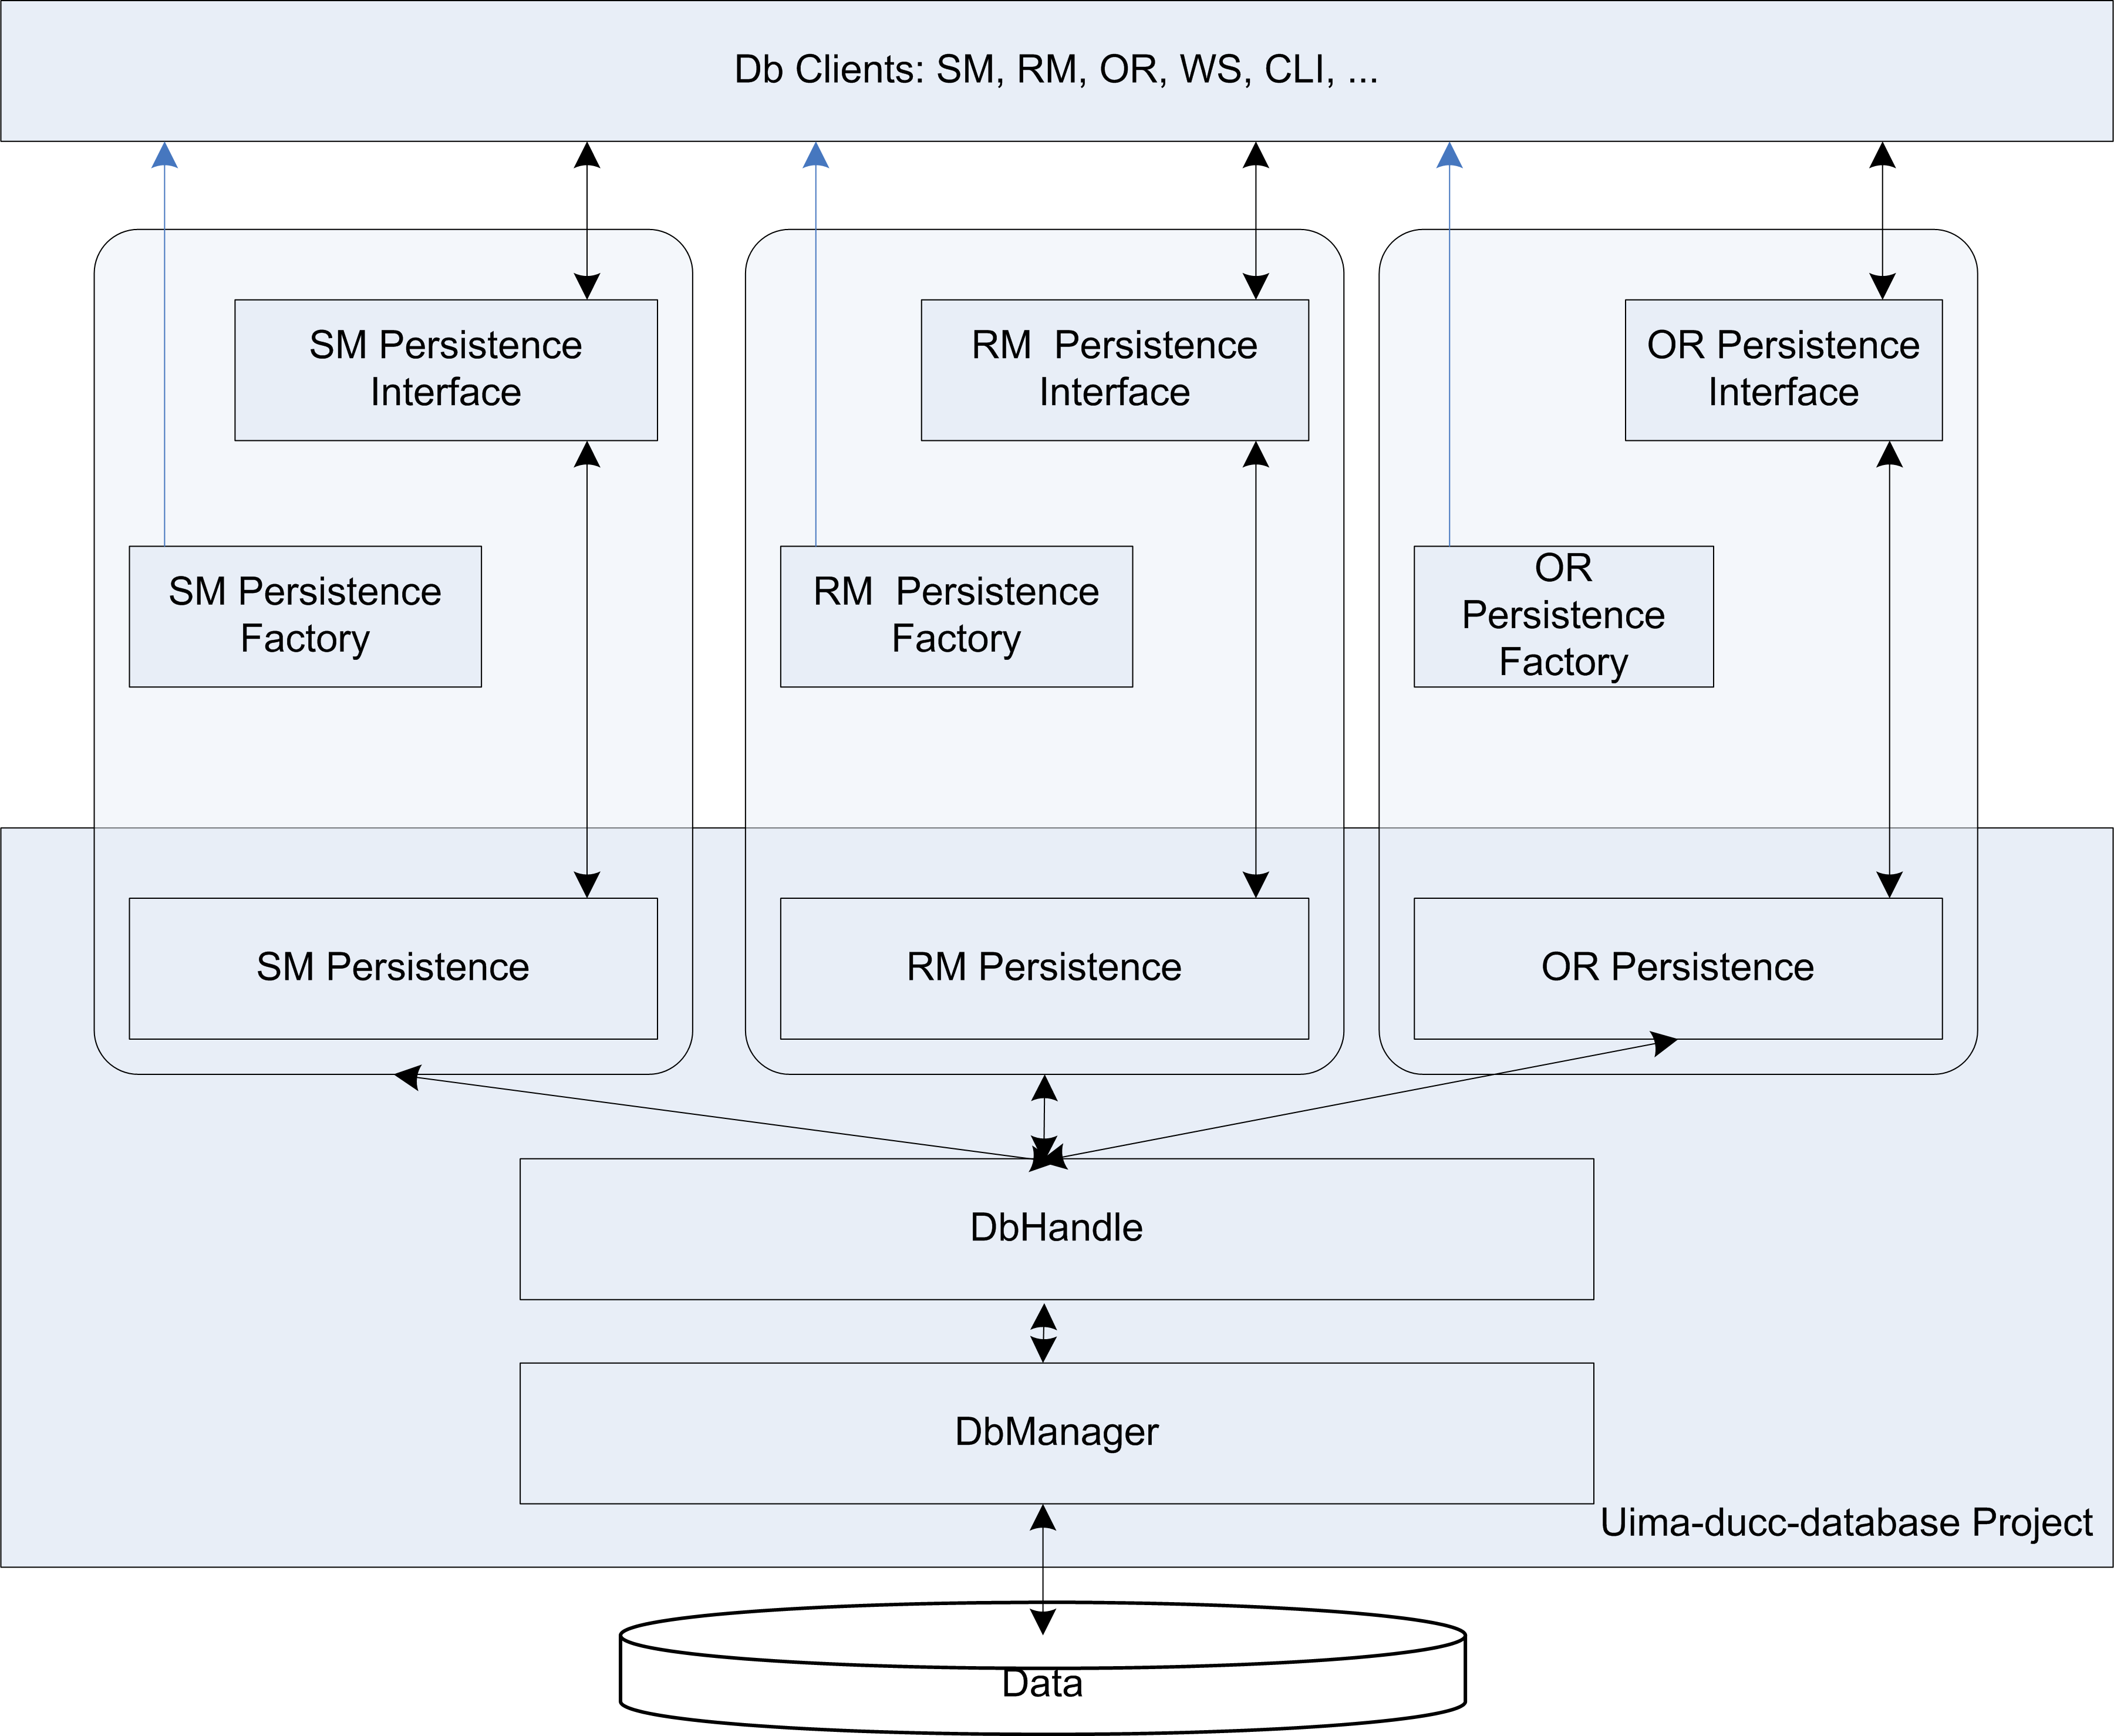
\includegraphics[width=5.5in]{images/ducc-internals/db-structure.png}
      \caption{Database Structure}
      \label{fig:db-structure}
    \end{figure}


    Runtime dependencies are resolved with reflection.  Entries in ducc.properties
    are used to specify the classes which interface with the database.  The DUCC scripting
    insures that the CLASSPATHs of components using the database contain the 
    necessary entries.

    \paragraph{Factories}
    The Cassandra Java client is thread-safe and manages connection pooling.  Only a single
    Cassandra {\em session} should be acquired for all threads in a process.  To enforce this
    the {\em Factory} pattern is used to acquire database handles.  The factory creates
    a single static handle and returns this singleton on every call.

    The objects returned by the factories are referenced through their interfaces that describe all
    legal actions against the persistent store. 

    There are three factories:
    \begin{description}
      \item[HistoryFactory.java] This resides in 
\begin{verbatim}
uima-ducc-transport/src/main/java/org/apache/uima/ducc/transport/event/common/history
\end{verbatim}
        This is used by the Orchestrator to write history files and its checkpoint, and to restore
        the checkpoint on startups.  It is used by the Web Server to read work history.
      \item[StateServicesFactory.java] This resides in 
\begin{verbatim}
uima-ducc-common/src/main/java/org/apache/uima/ducc/common/persistence/services
\end{verbatim}
        This is used by the Service Manager to maintaining service registrations, service metadata,
        and service registration history.  It is used by the Web Server to show the service
        registration and meta details.
      \item[RmPersistenceFactory.java] This resides in
\begin{verbatim}
uima-ducc-common/src/main/java/org/apache/uima/ducc/common/persistence/rm 
\end{verbatim}
        This is used by the Resource Manager to maintain its internal scheduling state for the
        purpose of inspection by other agents.  This is used by the Web Server to show machine
        details.  This is used by the admin CLI to show the state of all machines and work in the
        system.
    \end{description}
    
    \paragraph{Interfaces}
    All higher-level communication to the database is done through objects returned from the
    factories which must conform to specific interfaces.  There are three interfaces:
    
    \begin{description}
      \item[IHistoryPersistenceManager.java] This resides in 
\begin{verbatim}
uima-ducc-transport/src/main/java/org/apache/uima/ducc/transport/event/common/history
\end{verbatim}
        See its Javadoc for details of its calling sequence.
      \item[IStateServices.java] This resides in
\begin{verbatim}
uima-ducc-common/src/main/java/org/apache/uima/ducc/common/persistence/services
\end{verbatim}
      See its Javadoc for details of its calling sequence.   
      \item[IRmPersistence.java] This resides in 
\begin{verbatim}
uima-ducc-common/src/main/java/org/apache/uima/ducc/common/persistence/rm
\end{verbatim}
      See its Javadoc for details of its calling sequence.
    \end{description}

    In addition to the calling sequences, these interfaces contain Java {\em enum} structures that
    describe the database schema.  See below for how these enums are designed.

    \paragraph{Implementations}
    Multiple implementations of each interface are provided.  In all cases, a ``null''
    implementation for which all methods are empty stubs is used as a fallback in the event that a
    more functional interface cannot be provided.  There are both {\em file-based} and {\em
      database-based} implementations for Orchestrator state and for the Service registry.  Resource
    manager state is provided via the database only.  See the DuccBook for details on how to select
    a specific implementation at runtime.

    In the case of the implementations that interface with the database, an additional method is
    required, but is not part of the public interface:
\begin{verbatim}
   static RETURN-TYPE mkSchema();
\end{verbatim}
    The specific type of object returned by this method varies with database implementations.  It
    must return a collection of objects that the database creation methods can use to create the
    database schema.
    
\section{Database Schema}
    The schema for all tables is controlled by Java {\em enum} objects in the various interfaces.  These enums must adhere to a specific
    interface, defined in
\begin{verbatim}
     uima-ducc-common/src/main/java/org/apache/uima/ducc/common/persistence/IDbProperty.java
\end{verbatim}

     There are five methods defined in this interface, used by the database package to automatically generate
     the schema.  These interfaces may also be used by applications when querying the database to determine
     the types and actual database column names for each table.

     Most elements in the enum define columns of a table in the database.  Methods on the enum
     contain meta-data required to correctly create and interpret the data in a column.  Some elements in the
     enum are meta-data about the column itself.

     These methods are:
     \begin{description}
       \item[String pname()] This the name of a column as known by DUCC and may contain any ASCII
         characters.  Note this need not be the name of the column in the database.
       \item[String columnName()] This is the name of the column as used in the database.  It must
         conform to the column-naming standards of the database being used.  
       \item[Type type()] This specifies the type of data in the column.  Rather than specifying the
         database-specific type names, we supply an abstract name in the Type object which the
         database package translates to the correct form for the specific database implementation.
       \item[isPrimaryKey()] If true, the data in the column defined by this enum is a primary key.
         It is legal to specify multiple columns as primary keys, in which case, the database
         component will create a compound primary key.  The keys are generated in the order
         they occur in the enum.
       \item[boolean isPrivate()] This enum element is used by the database package only and
         should never be passed back to applications.  It allows the
         database package to maintain table-specific information that is not accidentally 
         translated into a return element. For example this is used when a row corresponds to
         a collection of Java properties, but the enum does not correspond to one of the
         returned properties.
       \item[boolean isMeta()]  This is the converse of isPrivate().  This allows
         an application to pass information to the database component that does not get
         placed into the schema or database.  For example, the name of the table may be
         defined in the enum, but this should not become the name of a column in any table.
       \item[isIndex()] If {\em true}, this column is indexed in the schema.  Multiple columns
         may be specified for indexing.
       \end{description}
     
     \paragraph{Types} We maintain a level of indirection between DUCC and specific database types, to enable
     disparate database implementation from a common meta-schema.  The DUCC-defined database
     types are:

     \begin{description}
       \item[String] The database implementation translates this into the appropriate
         type for the database, for example, {\em varchar} for a DB2 database.
       \item[Blob] This specifies a binary large object, e.g. a serialized
         Java object.
       \item[Integer] This specifies a 32-bit integer.
       \item[Long] This specifies a 64-bit integer.
       \item[Double] This specifies a Java object of type {\em double}
       \item[UUID] Some modern databases have native support for Java UUIDs.  This specifies
         an object conforming to that type.  Older databases may translate this to {\em char}
         or {\em varchar}.
     \end{description}
     
\section{The uima-ducc-database package}
     This package is intended to be isolated as much as possible from the rest of DUCC.  The
     design-point is that it should be mostly straightforward to change the database implementation,
     or to create additional persistence implementations, as long as the functions described
     in the previous sections are maintained.

     \paragraph{Database Core} Most of the database interface is contained in two classes:
     \begin{description}
       \item[DbManager] This object is responsible for directly interfacing with the
         specific database implementation.  It knows how to manage the
         database URL, how to contact the database, how to execute commands (e.g. SQL)
         against the database, how to create users and manage security, and the
         general structure of the DB API.

         This object is to be used only to initiate database communication. It generally does not
         know much about the specific query language used (e.g. CQL vs SQL), which is left to the
         DbHandle.
       \item[DbHandle] This provides a level of indirection between {\em clients} of the
         database, and the {\em implementation} of the database.  A {\em client} 
         instantiates a DbManager and then requests a {\em DbHandle} whenever it actually
         needs to communicate to the DB.  If session pooling is supported, the DbHandle should
         transparently enable this so higher-level layers need not be concerned with it.

         The handle rarely communicates directly with the database itself.  Instead, it 
         requests the DbManager that created it to do actual communication.
     \end{description}

     \paragraph{Bootstrap modules} Some specialized functions are separated into discrete classes:
     \begin{description}
       \item[DbAlive] This module communicates directly with the database, bypassing both
         the DbManager and DbHandle.  It is considered a {\em bootstrap} object.  It assumes
         the database has been started, and attempts to contact it, determine if the
         {\em ducc} and {\em guest} userids are defined, and queries the schema.  This
         implements retry logic as the database can take time to start up.  It bypasses
         the DbManager because if the database is in some way compromised, it may not be
         possible to successfully instantiate a DbManager or DbHandle.
       \item[DbCreate] This module also bypasses the DbManager and communicates directly
         with the database.  It creates the {\em ducc} superuser id, disables the
         default superuser, and creates a restricted {\em guest} userid.

         This is also considered a bootstrap object.
       \item[DbLoader] This module is used to load an existing DUCC file-based {\em history,
           checkpoint,} and {\em service registry} into the database.  It is considered a bootstrap
         module and communicates directly to the database when it can for best performance, and and
         indirectly through the implementations of the DUCC persistence objects to create summary
         tables of the various objects.
     \end{description}
     
     \paragraph{Schema Creation}
     Each of the DUCC-component-specific database implementations must implement a method
\begin{verbatim}
   static RETURN-TYPE mkSchema();
\end{verbatim}
     where the {\em RETURN-TYPE} depends on the specific database implementation.  In the case
     of Cassandra, the full signature is
\begin{verbatim}
   static List<PreparedStatement mkSchema();
\end{verbatim}

     The DUCC-component implementations inspect their schema definitions, as defined in the
     IDbProperty enums in their interfaces, and create, in the case of Cassandra, a collection
     of PreparedStatements which the {\em DbCreate} then uses to generate schema.

     \paragraph{Utility Modules}
     \begin{description}
       \item[DbUtil] This contains common, static, methods that know how to manipulate
         the IDbProperty enums to create schemas, indexes, convert property files into
         {\em INSERT / UPDATE} statements, and so on.
       \item[RmNodeState] This is example code that demonstrates one way to query the database
         and generate a {\em json} object of current Resource Manager state for clients.
       \item[RmQLoad] This is example code that demonstrates one way to query the database
         and generate a {\em json} object of current Resource Manager demand for clients.
     \end{description}
     
     \paragraph{DUCC component-specific implementations}
     These modules implement persistence for the Orchestrator, Service Manager, and Resource
     Manager, implementing their indicated interfaces as well as the required {\em mkSchema}
     methods.  They should never be directly accessed outside of the database package.  Instead,
     they must be instantiated by the correct {\em Factory} as described in earlier sections.

     \begin{description}
       \item[HistoryManagerDb]This implements persistence for Orchestrator-generated
         history and checkpoint.  
       \item[StateServicesDb] This implements persistence for the Service Manager's
         registry and history.
       \item[RmStatePersistence] This implements persistence for the Resource Manager's
         dynamic state.

         Note that this state is always deleted whenever RM initializes or reconfigures,
         and is rebuilt as the RM itself builds or recovers its dynamic state.
       \end{description}

\section{Tables}
    This section describes all of the tables.


    \paragraph{HistoryManagerDb} The {\em HistoryManagerDb} module is responsible for the
    schema and maintenance of the tables used for most of the history objects and the
    Orchestrator checkpoint.

       \begin{description}
          \item[job\_history] This contains the serialized objects for all Job history as {\em BLOB}s. 
          \item[res\_history] This contains the serialized objects for all Reservation history as {\em BLOB}s.
          \item[svc\_history] This contains the serialized objects for all Service history as {\em BLOB}s.
          \item[orckpt] This contains the Orchestrator checkpoint.  There are two {\em BLOB}s in this object:
            the current OR map, and the job-to-process map.
          \item[jobs] This contains details for all jobs, extracted from the {\em BLOB}s that are written
            to {\em job\_history}.  It does not include any process history however.
          \item[processes] This contains details for all objects that get allocated space by the RM:
            job processes, service processes, AP processes.
          \item[reservations] This contains details for all reservations, extracted from the {\em BLOB}s that are written
            to {\em res\_history}.
       \end{description}

   \paragraph{StateServicesDb} The {\em StateServicesDb} module is responsible for the 
   service registry.  

   \begin{description}
     \item[smreg] This contains the service registrations as submitted by users.
     \item[smmeta] This contains active state of services.
   \end{description}

   \paragraph{RmStatePersistence} The {\em RmStatePersistence} module is responsible for all the
   dynamic state produced by the RM.

   \begin{description}
     \item[rmnodes] This contains the state of all nodes known to the RM.
     \item[rmshares] This contains details on all the shares currently allocated by RM.
     \item[rmload] This contains the ``demand'' on the RM: counts of all services that are 
       requested by jobs, and counts of services RM is able to satisfy. (The intended purpose
       of this table is to allow external agents to inspect RM load and in conjunction with
       rmnodes and rmshares, determine whether RM is under-, over-, or sufficiently provisioned.)
   \end{description}
   
\section{Scripting and Configuration}
    The goal of the DUCC scripting support for the database is to make database start-up, shutdown,
    schema initialization, migration, and configuration as transparent as possible.  

    \paragraph{Configuration} Here we define {\em configuration} to refer to the files 
    that define the database URL, the hosts it may be running on, the
    location of the physical data, etc.  A number of these values are determined
    by virtue of the way DUCC and the database are designed to work together.  

    There are two relevant files. Pre-configured versions of these file reside in the
    DUCC source base in the directory
\begin{verbatim}
src/main/resources
\end{verbatim}

    During system build these files are copied into the database configuration
    directory.

    Note that if the database is updated or replaced it will generally be required
    to  obtain re-configure these files and replace them in the build directory.

    The files are:
    \begin{description}
      \item[cassandra.yaml] This is the primary configuration file.  Details of its
        contents are found in the standard Cassandra documentation.  We prepare this
        configuration thus:
        \begin{itemize}
          \item Set the database {\em cluster name} to DUCC.
          \item Set the hostname where the Cassandra server resides in three places:
            the {\em seed\_provider}, the {\em listen\_address}, and the {\em rpc\_address}.
            The reconfigured {\em cassandra.yaml} sets these all to the constant string
            {\em DUCCHOST}; the DUCC startup scripting changes these to the value of
            {\em ducc.head} before starting Cassandra.
          \item Set the authentication scheme to {\em PasswordAuthenticator} to force
            userid and password access.
          \item Set the authorizer module to {\em CassandraAuthorizer} to enable specific
            permissions to be set on the configured userids.
          \item Set the location of the database files in {\em data\_file\_directories}.
          \item Set the location of the database commitlog in {\em commitlog\_directory}.
          \item Set the location of the database saved caches in {\em saved\_caches\_directory}.
        \end{itemize}
      \item[cassandra.env.sh] This is a shell script that is run by Cassandra as it is
        starting up to detect the environment and set its internal parameters. The following
        DUCC changes are applied:
        \begin{itemize}
          \item Alter checks for the JVM vendor so it will start with the IBM JVM.
          \item Parameterize some things so the can be pulled from the environment, and
            thus enable Cassandra to be customized from {\em ducc.properties}.  The following
            items have been modified in this file for this purpose: JMX\_PORT.  (Note that
            {\em Xmx and Xms} are already customizable by setting environment variables.)
        \end{itemize}
      \end{description}
    
      \paragraph{Scripting}
      
      
      \paragraph{} 

      The following updates to the DUCC scripting support the database:
      \begin{description}
         \item[ducc.head Configuration] When DUCC is started, a small bit of code is executed to insure
           the {\em ducc.head} node is properly configured in the Cassandra configuration {\em
             cassandra.yaml}.  If not, a message is emitted and the configuration file is updated
           before attempting to start DUCC.
        \item[ducc\_util.py] This contains common database routines used by all scripts that extend
          the base class {\em DuccUtil}.  These methods perform these functions:
          \begin{description}
            \item[Enable DB] db\_configure reads {\em ducc.database.host} and if it is set to
              ``--disabled--'', a global variable is set to indicate the DB is disabled.  Otherwise
              it reads the database password from {\em ducc.private.properties} and sets that into
              a global variable.  If there is no password set, the DB is set disabled regardless of
              the value of {\em ducc.database.host}.
           \item[DB process running] db\_process\_alive attempts to determine if the database process
             is running (which is not equivalent to the database being functional).
           \item[DB functional] db\_alive attempts to contact the database by calling the Java bootstrap
             routine ``DbAlive'' (see previous section).  It returns true or false to indicate whether
             the DB appears functional.
           \item[DB stop] db\_stop uses the Cassandra pid to send {\em kill -TERM} to stop the DB process.
           \end{description}
         \item[db\_util.py] This contains database methods that can be called from any scripting that
            need not extend {\em DuccUtil}.  It contains methods to stop the database, update 
            {\em cassandra.yaml} with the value of {\em ducc.head}, and assist parsing and formatting
            the results of executing {\em cqlsh}.
          \item[ducc.py] This contains a method to start Cassandra.  It is called from {\em start\_ducc}
            and {\em startsim}.
          \item[start\_ducc] This contains calls to {\em ducc\_util.py}  and {\em ducc.py} to configure
            and start the DB, and then insure it comes up before starting the rest of DUCC.
          \item[stop\_ducc] This contains calls to {\em ducc\_util.py} to stop the DB.
          \item[check\_ducc] This contains calls to {\em ducc\_util.py} to determine if the DB is running or not.
          \item[ducc\_post\_install] This contains calls to {\em db\_util.py} to configure the
            {\em ducc.head}, generate a random database password, and initialize the schema.
          \item[db\_create] This contains methods to define a database, independently of
            {\em ducc\_post\_install} intended for migration purposes.
          \item[db\_loader] This contains calls to the java utility {\em DbLoader} to
            migrate existing state and history files to the database.
          \item[startsim] This contains calls to {\em ducc\_util.y} to start the database and
            insure it starts correctly.
          \item[stop\_sim] This contains calls to {\em ducc\_util.y} to stop the databse.
          \end{description}
          

